\chapter{Fed-Safe: Securing Federated Learning in Healthcare Against Adversarial Attacks}
\begin{abstract}
    
\dropcap{F}ederated learning is a popular technique for medical image analysis, due to its promise of high accuracy with limited communication overhead. However, federated learning suffers from privacy and security issues. As an example, malicious clients might be able to acquire sensitive information from other clients or disrupt the training process. Such challenges hamper the large-scale deployment of federated learning networks in medical image applications.  This paper proposes a novel approach to improve the robustness of federated learning networks against adversarial attacks. Secure aggregation is utilized to protect the privacy of data owners, while various techniques such as homomorphic encryption and differential privacy are used to reduce the risk of attack. Moreover, a model based on federated adversarial adaptation is proposed, incorporating distributed noise to secure downlink requirements. Experiments are conducted to demonstrate the efficacy of this system in comparison to baseline models, resulting in improved security against malicious clients, as well as satisfactory accuracy.
\end{abstract}
\newpage
\lettrine{F}{} ederated learning is a popular technique for medical image analysis, due to its promise of high accuracy with limited communication overhead. However, federated learning suffers from privacy and security issues. As an example, malicious clients might be able to acquire sensitive information from other clients or disrupt the training process. Such challenges hamper the large-scale deployment of federated learning networks in medical image applications. 
\marianna{Here's a sample comment from Marianna}
\\To increase the robustness of federated networks against adversarial attacks, various methods such as secure aggregation, homomorphic encryption, and differential privacy have been employed. Secure aggregation utilizes the fact that a client's individual data can be protected by not collecting the entire dataset. This technique allows for the querying of personal data without jeopardizing the data owner's privacy, as random noise is added to the dataset of each client. \peter{Peter M.A.: Try to condense this, it doesn't flow and is too complicated.

}Despite this, other studies have demonstrated that these models are highly sensitive to adversarial attacks due to the trade-off between privacy and security. Furthermore, the purpose of these methods is more to provide privacy, rather than security, thus leaving the models highly vulnerable to adversarial attacks.
\\In this paper, we propose an enhanced approach to defending against adversarial attacks in federated learning. After federated training is completed using differentially private methods, the central server adds a number of synthetic adversarial examples and performs an optimization causing federated adversarial adaptation. The resulting model is then sent to the clients with added Gaussian noise, also known as distributed noise, which satisfies the downlink requirements for DP. This approach \peter{.: what are downlink requirements? and what is DP, abbreviation hasn't been explained before
 } reduces the chance of successful adversarial attacks and improves the security of the federated network. \peter{Peter M.A.: This should not be part of the introduction. It is more a discussion paragraph. In the introduction you don't describe results of your work.
}Experimental results demonstrate that our proposed system is robust against malicious clients, while still providing satisfactory accuracy when compared to unsecured baseline models.
\\Our proposed system is highly resilient to adversarial attacks and has a significant impact on the robustness of the federated learning networks. Distributed noise allows us to protect the data sets of each local client without compromising the privacy guaranteed by differential privacy. Additionally, our framework is not limited to a single attack scenario but is capable of defending against a variety of adversarial attacks. Experimental results show that our system achieves satisfactory accuracy compared to unsecured baseline models, as well as better performance than both differential privacy and baseline adversarial training methods, while providing improved security against malicious clients 
\section{Related works}
While there are published research studies on federated learning for
medical images, as well as on adversarial attacks on medical images in centralised settings, to
the best of the authors’ knowledge, our work is the first to propose a federated learning system with robustness to adversarial attacks.

\textbf{Federated Learning for Medical Image Analysis.} Federated learning has been  explored in multiple studies for medical image analysis. For instance, Liu et al. proposed a federated learning system for medical image classification that achieved an accuracy of 89.17\% on the Chest X-Ray dataset, using multiple hospitals as clients\cite{liu2020experiments}. Similarly, Malik et al. proposed a secure federated learning framework for medical image classification, using a secure multi-party computation protocol for secure aggregation and achieving an accuracy of 98.45\% on the Chest X-Ray dataset\cite{malik2023dmfl_net}.




\textbf{Adversarial Attacks on Medical Images.}  Studies have shown that medical images are vulnerable to adversarial attacks in a centralized setting. For instance, Han et al. \cite{han2020deep} proposed a deep learning-based system for classifying cardiac diseases from ECG signals and assessed its vulnerability to various white-box and black-box adversarial attacks. Similarly, Rodriguez et al.'s proposed system for classifying chest x-ray abnormalities \cite{rodriguez2022role} was found to be highly vulnerable to different types of adversarial attacks. Bortsova et al. further studied the adversarial attacks and detection of medical images within a centralized setting \cite{bortsova2021adversarial}.

\textbf{Secure Federated Learning}  (SFL) has been widely studied, with research focusing on both privacy and robustness. For example, So et al. proposed a secure aggregation protocol for SFL to protect against various attack scenarios \cite{so2022lightsecagg}. Chen et al. presented an end-to-end secure aggregation protocol to maintain client privacy while preserving model accuracy \cite{chen2022poisson}. Studies concerning encryption and privacy-preserving approaches, such as differential privacy, have also been conducted. Ma et al., for instance, proposed a front-end framework using multi-key encryption \cite{ma2022privacy}, while Zhang et al. created a platform using homomorphic encryption for secure aggregation without considering DP or encrypted inference \cite{zhang2022homomorphic}. Sheller et al. implemented a privacy-preserving FL segmentation model without using DP or assessing its robustness\cite{sheller2020federated}, Vithana et al. showcased a segmentation task but relied on a different technique (sparse vector) instead of DP \cite{vithana2022model}, and Adnan et al. provided a framework for FL with differential privacy concerning pathology slides without covering secure aggregation or encrypted inference \cite{adnan2022federated}. Adversarial training has been applied as an optimization technique for individual clients in order to secure federated networks; however, this also increases computational burden for all participants, potentially leading to lack of convergence due to heterogeneity among models \cite{bagdasaryan2020backdoor}.
\section{Proposed method}

 \subsection{Model Aggregation}
 In this section, we discuss the Model Aggregation method used in federated learning scenarios. Federated learning networks involve multiple clients from which the central server collects updates and performs aggregation. The aggregation model adopted for this situation is Federated Averaging, though the defense technique referenced herein applies to any other aggregation model. In contrast to standard federated averaging, the central server undertakes more processing to  enforce adversarial robustness, which is explained in further detail in the following sections.\\ To ensure the privacy of updates to our model, we propose distributed noisy communication channels. Our proposed model, satisfies the global $(\epsilon, \delta)$-DP requirement, in both uplink and downlink channels. 
We utilize a clipping method for the uplink which bounds each clients' training parameters $\mathbf{w}_{i}$ with a value of $C$. We assume that the batch size is equal to the number of training samples and then define the local training process for the $i$-th client:
\begin{equation}
\label{localtrain}
{s}_{\text{U}}^{\mathcal D_i}\triangleq \mathbf{w}_{i}=\arg\min\limits_{\mathbf{w}}{F_{i}(\mathbf{w}, \mathcal D_i)}=\frac{1}{\vert \mathcal D_i \vert}\sum_{j = 1}^{\vert \mathcal D_i \vert}\arg\min\limits_{\mathbf{w}}{F_{i}(\mathbf{w}, \mathcal D_{i,j})},
\end{equation}
where $\mathcal D_i$ is the $i$-th client's database and $\mathcal D_{i,j}$ is the $j$-th sample in $\mathcal D_i$. Thus, the sensitivity of $s_{\text{U}}^{\mathcal D_i}$ can be expressed as
\begin{multline}\label{SensitivityforUP}
\Delta s_{\text{U}}^{\mathcal D_i} =\max_{\mathcal D_i, \mathcal D_i'}{\Vert s_{\text{U}}^{\mathcal D_i}-s_{\text{U}}^{ \mathcal D_i'}\Vert}
=\max_{\mathcal D_i, \mathcal D_i'}\left\Vert \frac{1}{\vert \mathcal D_i \vert}\sum_{j = 1}^{\vert \mathcal D_i \vert}\arg\min\limits_{\mathbf{w}}{F_{i}(\mathbf{w}, \mathcal D_{i,j})}\right.\\
\left.-\frac{1}{\vert \mathcal D_i' \vert}\sum_{j = 1}^{\vert \mathcal D_i' \vert}\arg\min\limits_{\mathbf{w}}{F_{i}(\mathbf{w}, \mathcal D_{i,j}')}\right\Vert= \frac{2C}{\vert \mathcal D_i \vert},
\end{multline}
where $\mathcal D_i'$ is an adjacent dataset to $\mathcal D_i$ which has the same size but only differ by one sample, and $\mathcal D_{i,j}'$ is the $j$-th sample in $\mathcal D_i'$.

From the above result, a global sensitivity in the uplink channel can be defined by
\begin{equation}
\Delta s_{\text{U}}= \max\left\{\Delta s_{\text{U}}^{\mathcal D_i}\right\},\quad\forall i.
\end{equation}

To minimize the sensitivity, all clients must have sufficiently large datasets for training, prompting us to define the minimum size of the local dataset as $m$ and obtain $\Delta s_{\text{U}} = \frac{2C}{m}$.
For each client to consider one $(\epsilon, \delta)$-DP in the uplink channel, we specify the noise scale, symbolized by the standard deviation of the additive Gaussian noise, to $\sigma_{\text{U}}= c\Delta s_{\text{U}}/\epsilon$.
Considering the $L$ exposures of local parameters, we have to set $\sigma_{\text{U}}= cL\Delta s_{\text{U}}/\epsilon$ due to the linear relation between $\epsilon$ and $\sigma_{\text{U}}$ in the Gaussian mechanism. 




When looking at the downlink channel, the aggregation of $\mathcal D_i$ can be expressed as
\begin{equation}
\label{DLfunction}
s_{\text{D}}^{\mathcal D_i}\triangleq \mathbf{w}=p_1\mathbf{w}_{1}+\ldots+p_i\mathbf{w}_{i}+\ldots+p_N\mathbf{w}_{N},
\end{equation}
where $1\leq i\leq N$ and $\mathbf{w}$ is the merged parameters that the server broadcasts to its clients. Throughout this, there is a balance between privacy and security.

\subsection{Distributed noise}
Some methods impose strict privacy regulations. Although this helps keep sensitive information private, there's always a trade-off between privacy and security against adversarial attacks. 

 In order to protect sensitive data while still providing a safe environment against adversarial attacks, our distributed noise model presents a two-part solution. First, we generate a series of synthetic examples to perform adversarial adaptation on the global server. Additionally, we add distributed gaussian noise to the downlink channels to the client. By minimizing the adversarial adaptation loss function, the network becomes resilient to potential adversaries that may be present in the clients. Furthermore, this method of noise-based protection does not interfere with local training. The benefit of the global model being re-trained is that it learns the distribution of all the clients' models, increasing its resilience to potential adversaries. Through the implementation of a distributed noise system, it is possible to secure both privacy and security.



\begin{algorithm}[h]
\caption{Federated adversarial adaptation}
\label{algo1}
% \begin{algorithmic}[1]
% % 
% \label{alg:ATFL}
% \LinesNumbered
$X \in \mathcal{X}$, $Y \in \{-1, 1\}$, $g_{\beta}$: $\mathcal{X} \to \{-1, 1\}$, $\epsilon$: privacy parameter, $\eta$: bound, $\alpha$: step size
\STATE Initialize parameters: $\beta = \beta_0$ and $T = 0$\\
\While{$T < T_{max}$}{\\
      \ForEach{client}{
        Perform local federated training with differential privacy \\ 
        $g_{\beta} \leftarrow g_{\beta_T}$
    }
    Aggregate the models from all clients to create the global model\\
        Update parameters: $\beta = \beta_{T+1}$ and $T = T+1$
}
 
    
    Generate adversarial examples using the global model:
    \begin{equation*}
    x_{adv} = x + \epsilon\ \mbox{sign}(\nabla_x\mathcal{L}(\theta,x,y)),
    \end{equation*}
    Perform federated adversarial adaptation $g_{\beta_{T+1}}$ with data set $X_T$, $Y_T$ by performing the following optimization: 
    \begin{equation*}
            g_{\beta_i} = \argmin_{g_{\beta}} \mathcal{L}(g_{\beta}, D_i \cup D_i^{adv}) 
        \end{equation*}
    \For {$k \in \{1,\dots,N\}$}{
     \STATE Add distributed noise $\mathcal{N}(0, \sigma^2)$ to $g_{\beta_{T+1}}$ \\
        \STATE Receive the noisy model $\hat{g}_{\beta_{T+1}}^{(k)}$ \\
    }
\end{algorithm}


\textbf{Generating Adversarial Examples}: In the clients, it takes the global model that it collects and takes a data set and updates it using the global model that is expressed as an advertisement. And it actually performs an optimization. The examples are generated using two methods, first FGSM,where the global model uses a test dataset, it generates examples.


\noindent{\emph{The Fast Gradient Sign Method} (FGSM)} generates an adversarial sample $x_{adv}$ from an individual input sample $x \in \mathcal{X}$ (where $\mathcal{X}$ represents a set of samples) in a single step, using the sign
of the gradient $\nabla$ of a loss function $\mathcal{L}$ of the network\cite{kurakin2018adversarial}:
%
\begin{equation} \label{eq:FGSM}
x^{adv} = x + \epsilon\ \mbox{sign}(\nabla_x\mathcal{L}(\theta,x,y)),
\end{equation}


where $\epsilon$ is a positive constant that determines the scale of the perturbation , and $\theta$ denotes the model parameters.



\noindent{\emph{Projected Gradient Attack} (PGD)\cite{madry2017towards,liu2022threats}} is a more powerful multi-step variant of FGSM:

% \begin{equation} \label{eq:PGD}
% x^{t+1} = \Pi_x+S(x^t + \alpha\ \mbox{sign}(\nabla_x\mathcal{L}(\theta,x,y)),
% \end{equation}
%\comZR{not sure what is S, so suggest another one:}
%\comGP{cool, let's go with yours}
\begin{equation} \label{eq:PGD}
x^{i+1} = \mbox{clip}(x^i + \alpha\ \mbox{sign}(\nabla_{x^i}\mathcal{L}(\theta,x^i,y)),
\end{equation}
where $i$ is the iteration step, and $\alpha$ is a constant value that affects the perturbation scale. The $\mbox{clip}(\cdot)$ function aims to clip the perturbations into a small interval, \ie $|\alpha\ \mbox{sign}(\nabla_{x^i}\mathcal{L}(\theta,x^i,y))|\leq \eta$, where $\eta$ is a positive constant. Compared to FGSM, PGD yields a number of possible adversarial samples in multiple iteration steps, but it has a higher computational complexity\cite{liu2022threats}.
Suppose every instance $x \sim D$ corresponds to a fixed label $y \in \{-1, +1\}$ and the label of $+1$ indicates that instance $x$ was generated by an adversary. To evade the classifier, adversary would generate an alternative instance $x' \in X$, for which $g(x') = -1$. 
Traditionally, machine learning algorithms commonly aim to minimize  empirical
risk:
\begin{equation}
\label{E:standardloss2}
\min_\theta \mathcal{L}(\theta) \equiv \sum_i l(g_\theta(x_i),y_i) 
\end{equation}


where $l(\hat{y},y)$ is the loss associated with predicting $\hat{y}$ when true classification is $y$, and $x_i$ and $y_i$ are the input feature vector and its corresponding label in the training data, respectively.
An important issue in adversarial settings is that instances
classified as malicious (in our convention, corresponding to
$g_\beta(x) = +1$) are associated with malicious agents who
subsequently modify such instances in order to evade the classifier
(and be classified as benign).
Suppose that adversarial evasion behavior is captured by an oracle,
$x^{adv}(\beta, x)$, which returns, for a given parameter vector
$\beta$ and original feature vector (in the training data) $x$, an
alternative feature vector $x'$.
\\\textbf{Federated Adversarial Adaptation}: After the adversarial examples are generated,
they are used to perform federated adversarial adaptation. The adaptation process follows optimizing of an augmented dataset, to train a robust model against 
adversarial attacks. The new model parameters are then sent to all the 
clients for evaluation.  Since the adversary modifies malicious instances according to this
oracle, the resulting effective risk for the defender is no longer
captured by Equation~\ref{E:standardloss2}, but must account for
an adversarial response.
Consequently, the global model would seek to minimize the following federated adversarial adaptation loss:
\emph{adversarial adaptation loss} (on training data):

\begin{equation}
\label{E:advloss}
\min_\theta \mathcal{L}_A(\theta; x^{adv}_{i}) = \sum_{i:y_i = -1} l(g_\theta(x_i),-1)+ \sum_{i:y_i = +1} l(g_\theta(x^{adv}_{i}(\theta,x_i),+1) 
\end{equation}
where $g_\theta(x)$ denotes the classifier output, $\mathcal{L}_A(\theta;  x^{adv})$ indicates the adversarial adaptation loss, and $ x^{adv}(\theta,x)$ represents any adversarial example that returns an alternative feature vector for input $x$ given parameter $\theta$.


The adversarial risk function in Equation~\ref{E:advloss} is extremely
general: we make, at the moment, no assumptions on the nature of the
attacker oracle, ${x^{adv}}$.
\\\textbf{Effect of adversarial adaptation}
To analyze what happens if the algorithm terminates, define the empirical risk in the last
iteration of federated adversarial adaptation as:
\begin{equation}
\label{E:radloss}
\mathcal{L}^R_N(\beta, {x^{adv}}) = \sum_{i \in D \cup N} l(g_\beta(x_i),y_i) 
\end{equation}
where a set $N = \cup_i N_i$ of data points has been added
by the algorithm.
We now characterize the relationship between $\mathcal{L}^R_N(\beta, {x^{adv}})$
and $\mathcal{L}_A^*({x^{adv}}) = \min_\beta \mathcal{L}_A(\beta,
{x^{adv}})$. Consequently, for any $\beta$ \begin{align*}
\mathcal{L}^R_N(\beta, {x^{adv}}) &\ge \mathcal{L}^R_N(\bar{\beta},
{x^{adv}})\\
&= \sum_{i: y_i = -1} l(g_{\bar{\beta}}(x_i),-1) +\sum_{i:y_i = +1} \sum_{j
  \in N_i \cup x_i} l(g_{\bar{\beta}} (x_i),+1) \\
&\ge \sum_{i: y_i = -1} l(g_{\bar{\beta}}(x_i),-1) +\sum_{i:y_i = +1}
l(g_{\bar{\beta}} ({x^{adv}}(\bar{\beta},x_i)),+1) \\
&\ge \min_\beta \mathcal{L}_A(\beta; {x^{adv}}) = \mathcal{L}_A^*({x^{adv}}),
\end{align*}
where the second inequality follows because in the last iteration of the algorithm, $new =
\emptyset$ (since it must terminate after this iteration), which means
that ${x^{adv}}(\beta,x_i) \in N_i$ for all $i \in I_{adv}$. This demonstrates how retraining the global model with adversarial examples can improve the robustness of the model against adversarial attacks. The proof shows that the  empirical risk in the last iteration of the algorithm is lower than the adversarial risk, and thus the model is more robust against adversarial attacks. 


% \begin{proposition}
% \label{prop:defender_loss_gen}
% Let $B = |I_{bad}|$.
% $\mathcal{L}_{A,01}^*(\mathcal{O}) \le \mathcal{L}^R_N(\beta,
% \mathcal{O}_L) + \delta(p)$ with probability at least $1-p$, where 
% % $\delta(p) = (p_L +
% % (-\frac{1}{2B} \log p)^{1/2})$, 
% $\delta(p) = B \left(p_L + \frac{\sqrt{\log^2 p-8 B p_l \log p}-\log p}{2B}\right),$
% and $\mathcal{L}^R_N(\beta,
% \mathcal{O}_L)$ uses any loss function $l(g_\beta(x),y)$ which is an upper bound on
% the $0/1$ loss.
% \end{proposition}

% \subsection*{Proof of Proposition 4.2}

% Let $\bar{\beta} \in \arg\min_{\beta}  \mathcal{L}^R_N(\beta,
% \mathcal{O}_L)$.
% Consequently, for any $\beta$,
% \begin{align*}
% \mathcal{L}_{A,01}^*(\mathcal{O}_L) &= \min_\beta \mathcal{L}_{A,01}(\beta;
% \mathcal{O}_L) \\
% &\le \sum_{i: y_i = -1} l_{01}(g_{\bar{\beta}}(x_i),-1) +\sum_{i:y_i = +1}
% l_{01}(g_{\bar{\beta}} (\mathcal{O}(\bar{\beta},x_i)),+1) + \alpha ||\bar{\beta}||_p^p.
% \end{align*}
% Now,
% \begin{align*}
% \sum_{i:y_i = +1} &l_{01}(g_{\bar{\beta}}
% (\mathcal{O}(\bar{\beta},x_i)),+1) \le \sum_{i:y_i = +1} l_{01}(g_{\bar{\beta}}
% (\mathcal{O}_L(\bar{\beta},x_i)),+1) + \delta(p)
% \end{align*}
% with probability at least $1 - p$,
% % where $\delta(p) = (p_L + (-\frac{1}{2B} \log p)^{1/2})$,
% where $\delta(p) = B p_L + \frac{\sqrt{\log^2 p-8 B p_l \log p}-\log p}{2}$,
% by the Chernoff bound, and Lemma~4.1, which assures that an
% optimal solution to Problem~(5) can only over-estimate mistakes.
% Moreover,
% \begin{align*}
% \sum_{i:y_i = +1} &l_{01}(g_{\bar{\beta}}
% (\mathcal{O}_L(\bar{\beta},x_i)),+1) \le\sum_{i:y_i = +1}\sum_{j \in N_i} l(g_{\bar{\beta}}
% (\mathcal{O}_L(\bar{\beta},x_i)),+1),
% \end{align*}
% since $\mathcal{O}_L(\bar{\beta},x_i) \in N_i$ for all $i$ by
% construction, and $l$ is an upper bound on $l_{01}$.
% Putting everything together, we get the desired result.

\include{proposed_method.tex}
\section{Experiments and Results}

\subsection{Datasets}
We employ non-IID datasets in our experiment, by creating chunks that represent a tiny portion of the general distribution, from which each client samples from exclusively. Two datasets are used to train the model - brain cancer classification, and histopathologic cancer detection. For brain cancer classification, 2870 training images and 394 test images are employed, while 1437 and 1426 training images are used to detect meningioma and glioma, respectively. For histopathologic cancer detection, 2150 samples are used,which are split 62\% for train and 38\% for the test. All images are transformed with flipping, rotation, and normalizing, and those for brain cancer classification are resized to 100$\times$100.
\subsection{Experimental Setup }
\\\textbf{Federated setup}:
A Convolutional Neural Network (CNN) with six layers of convolution stacks, five fully connected layers and ReLU activation function is used as the deep learning model (with 0.25 dropout parameter) to detect cancer in Histopathology images. The model is trained with Cross-Entropy loss via SGD optimizer. For federated setting, three clients equipped with random data with non-IID data distribution. FedAVG method is used to aggregate the models with 20 epochs per communication round and 50 federated rounds in total, weighed based on the size of the training dataset.
\\\textbf{Evaluation Metrics }:
We use two metrics to evaluate the performance of adversarial attacks, i.e. clean accuracy and attack success rate (ASR). Clean accuracy is defined as the performance of models on uncorrupted test images. Attack success rate (ASR) measures how much an adversary can change the predicted labels produced by each model. Formally, ASR is defined as:
\begin{equation}
    ASR = \frac{1}{N}\sum\limits_{i=1}^{N} (Pre\text{-}attack\;label_{i}\neq Post\text{-}attack\;label_{i})
\end{equation}
where $N$ is the number of images in the attack set. Attack accuracy (AA) shows the accuracy of an adversary after performing an attack, and transferability measures the effectiveness of attacks on different models.
\subsection{Results and analysis}
Our results show that distributed noise training provides superior defense against adversarial attacks compared to the adversarial training method. 
Across the three datasets, distributed noise training was able to reduce the attacker's self-ASR by up to 8\%, and the attacker's average ASR by up to 27\%, compared to the  adversarial training method (as shown in Table~\ref{tab:my_label}). This suggests that distributed noise is more effective at defending against adversarial attacks than the adversarial training method.

\begin{table}[]
    \centering
    \caption{Average values of ASR(self/avg) for different datasets as a result of distributed noise training and adversarial training technique. Lower value of ASR indicates a better defense against adversarial attacks.}
    \label{tab:my_label}
    \begin{tabular}{|l|l|l|l|}
\hline
Dataset & Step & \multicolumn{2}{l|}{Training Method} \\
& & Adversarial training & Distributed Noise \\
&& (ASR Self/Avg)& (ASR Self/Avg)\\\hline
\multirow{4}{*}{Glioma} & 0.005 & 0.03/0.00 & 0.03/0.00 \\ 
& 0.012 & 0.00/0.00 & 0.00/0.00 \\ 
& 0.017 & 0.00/0.00 & 0.00/0.00 \\ 
& 0.05 & 0.03/0.00 & 0.00/0.00 \\ \hline
\multirow{4}{*}{MRI} & 0.005 & 0.12/0.05 & 0.10/\textbf{0.02} \\ 
& 0.012 & 0.22/0.09 & 0.22/\textbf{0.08} \\ 
& 0.017 & 0.25/0.11 & 0.23/\textbf{0.04} \\ 
& 0.05 & 0.46/0.27 & 0.41/\textbf{0.15} \\ \hline
\multirow{4}{*}{Pathology} & 0.005 & 0.32/0.08 & 0.31/0.08 \\ 
& 0.012 & 0.43/0.12 & 0.47/\textbf{0.10} \\ 
& 0.017 & 0.46/0.17 & 0.49/\textbf{0.12} \\ 
& 0.05 & 0.54/0.32 & 0.65/0.34 \\ \hline
\end{tabular}
\end{table}

\vspace{30}
The effect of the perturbation parameter on the effectiveness of distributed noise was evaluated. The results, averaged over four experiments with and without differential privacy and with different re-training samples, showed that higher values of the perturbation parameter led to a higher attack success rate in all scenarios. Distributed noise consistently improved the performance of the adversarial training defense, with the greatest improvements seen in the Glioma dataset.
 In both defense models, the self-attack success rate (ASR) was around two to four times higher than the average attack success rate (ASR), indicating that the differences between the models in a federated learning network can lead to significant differences in the success of an attack. In contrast, the error rate of the undefended model was similar for the adversarial client and other clients, indicating high transferability of the attack.\\
\begin{table}[]
    \centering
    \caption{Effect of DP on the performance of distributed noise and adversarial training. The average attack success rate (ASR) values are shown for each dataset.}
    \label{tab:perturb_param}
    \begin{tabular}{|l|c|c|c|}

\hline
 & No DP & DP & \epsilon \\ \hline
Pathology & 10.21\% & 5.09\% & 0.01 \\
 & 9.97\% & 8.72\% & 0.03 \\
 & 9.53\% & 7.87\% & 0.05 \\
 & 19.04\% & 16.67\% & 0.07 \\
Average & 12.19\% & 9.58\% &  \\ \hline
MRI & 2.74\% & 0.31\% & 0.01 \\
 & 3.92\% & 0.32\% & 0.03 \\
 & 12.67\% & 0.32\% & 0.05 \\
 & 6.29\% & 0.32\% & 0.07 \\
Average & 6.41\% & 0.32\% &  \\ \hline
\end{tabular}
\end{table}
\\
\textbf{Effect number of adversarial adaptation samples}: Figure~\ref{fig: epsilon graphs} shows the effect of the number of adversarial adaptation samples on the performance of distributed noise and adversarial training.  The results, averaged over four experiments with and without differential privacy.We evaluate from 10,30,50,70 and 100 percent of the samples. showed that using more retraining samples in the global model led to a lower attack success rate in all scenarios. Using all of the training samples led to almost perfect defense in all scenarios, while distributed noise outperformed adversarial training and achieved perfect defense with much fewer samples, ranging from 10 to 70 percent.
\begin{figure*}[t!]
    \centering
     \begin{subfigure}
         \centering
         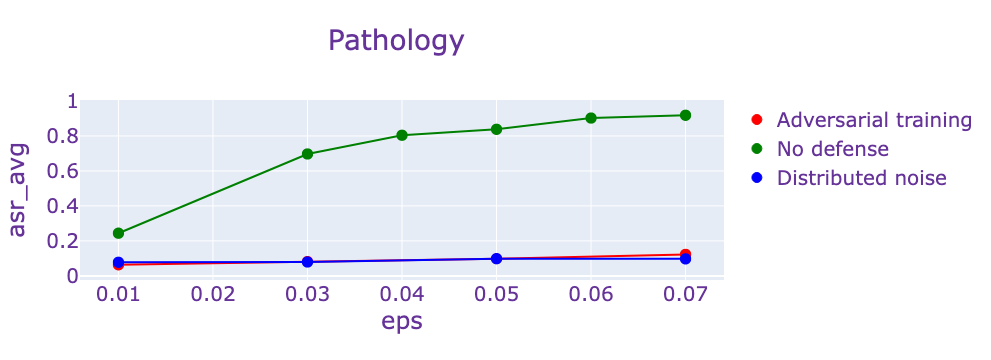
\includegraphics[width=0.55\textwidth]{newplot (22).png}\hspace{-60pt} 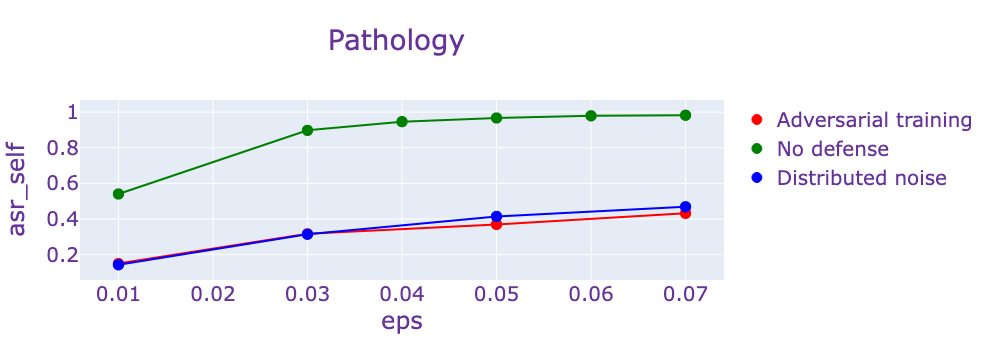
\includegraphics[width=0.55\textwidth]{newplot (21).png}
         % \caption{}
         \label{fig:AASR benign-EPS}
     \end{subfigure}
        \begin{subfigure}
         \centering
       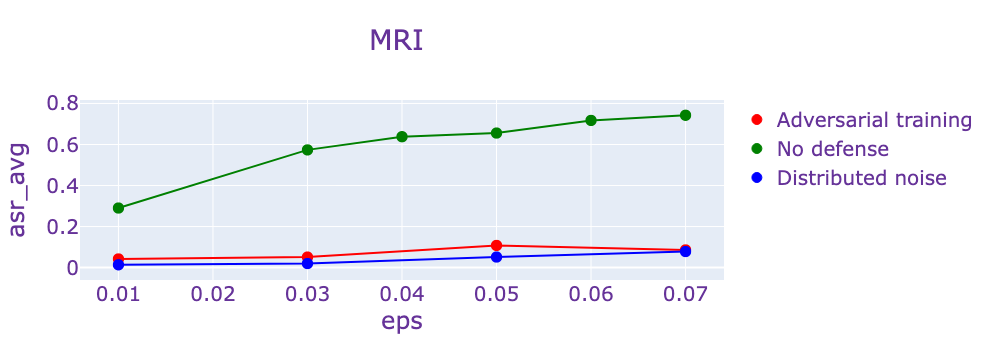
\includegraphics[width=0.55\textwidth]{newplot (20).png}\hspace{-60pt} 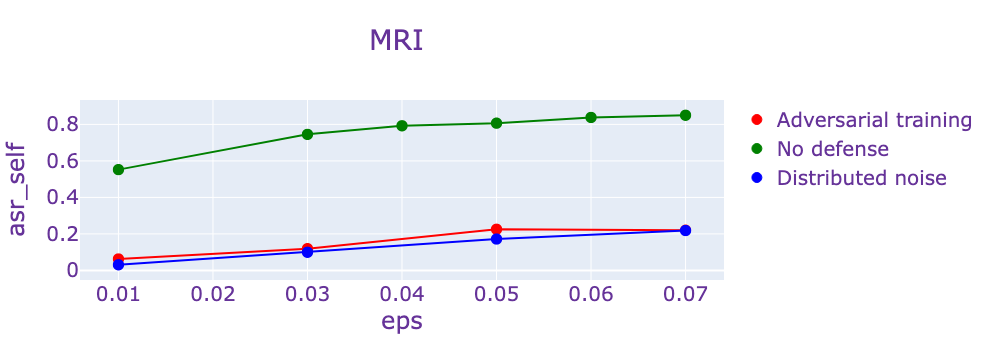
\includegraphics[width=0.55\textwidth]{newplot (19).png}
         % \caption{Effect of $\epsilon$ on Average ASR on benign clients }
         \label{fig:AASR benign-EPS}
     \end{subfigure}
     
      \centering
     \begin{subfigure}
         \centering
    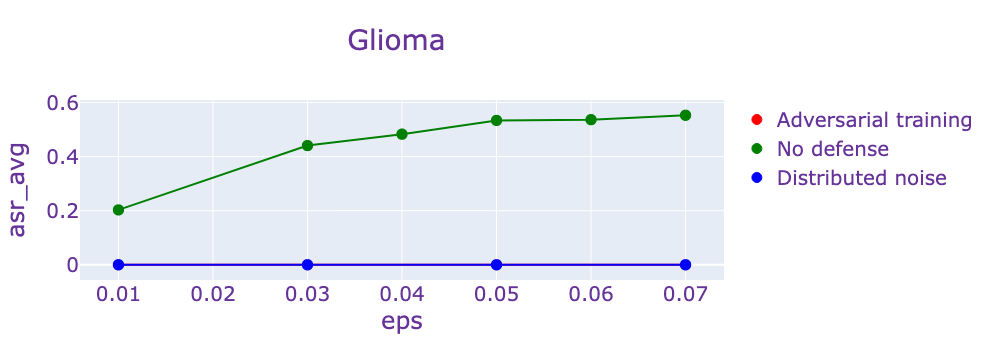
\includegraphics[width=0.55\textwidth]{newplot (18).png}\hspace{-60pt} 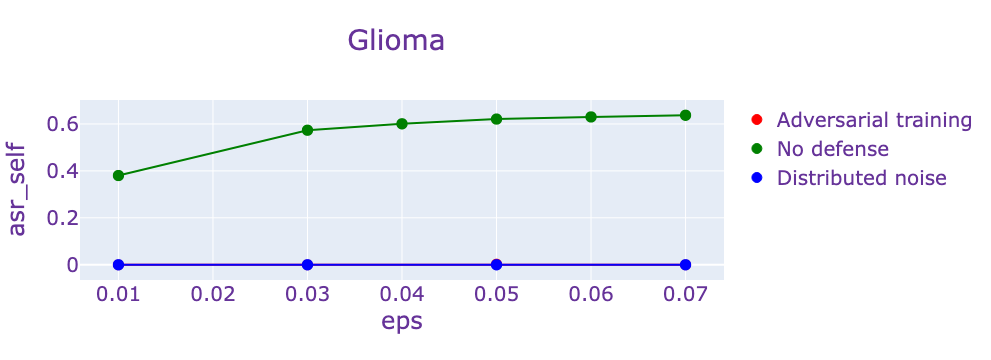
\includegraphics[width=0.55\textwidth]{newplot (17).png}
         % \caption{Effect of $\epsilon$ on Average ASR on benign clients }
         \label{fig:AASR benign-EPS}
     \end{subfigure}
     \hfill
        \caption{Effect of Error perturbation degree $\epsilon$ on attack transferability.PGD attack is performed.ASR is calculated on benign and adversary clients. The higher ASR on benign clients shows higher transferability}
        \label{fig: epsilon graphs}
\end{figure*}



\textbf{Effect of Differential privacy}:Table \ref{tab:perturb_param} shows the results of the experiments conducted to evaluate the effect of differential privacy on the defense methods. In both defense methods, adversarial training and distributed noise, DP reduced the average success rate (ASR) and hence improved the defense. For all attack values, the Glioma dataset resulted in perfect defense with ASR=0.0, and DP enabled defense for MRI was also almost perfect with both defense methods, resulting in average ASR= 0.31 percent. For the Pathology dataset, the average ASR was reduced from 12.19 percent to 9.58 percent when differential privacy was used. 

\begin{figure*}[t!]
    \centering
    \begin{minipage}{1.11\textwidth}
        \centering
        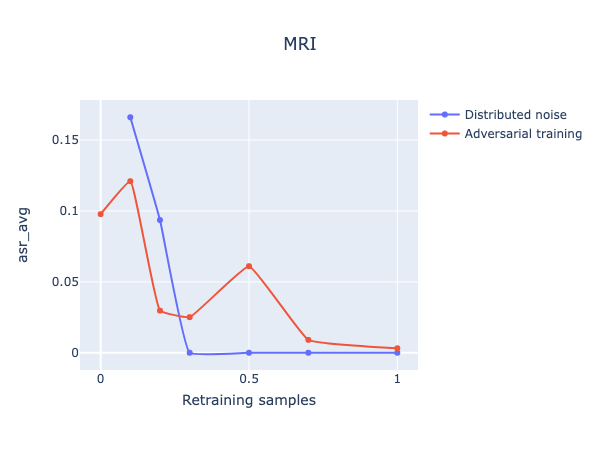
\includegraphics[width=0.55\textwidth]{newplot (14).png} 
        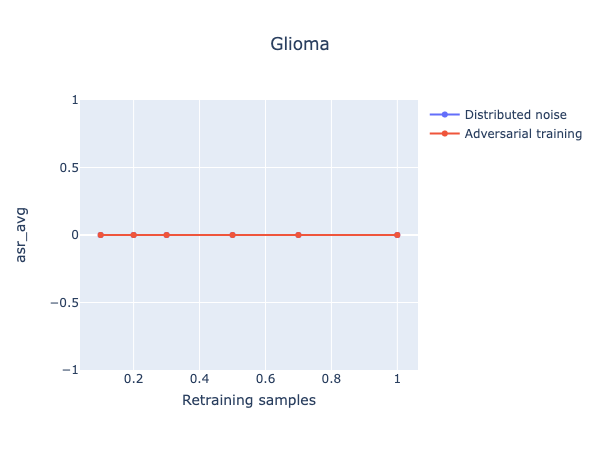
\includegraphics[width=0.55\textwidth]{newplot (12).png}\hspace{-40pt}
    \end{minipage}

    \begin{minipage}{1.21\textwidth}
        \centering
        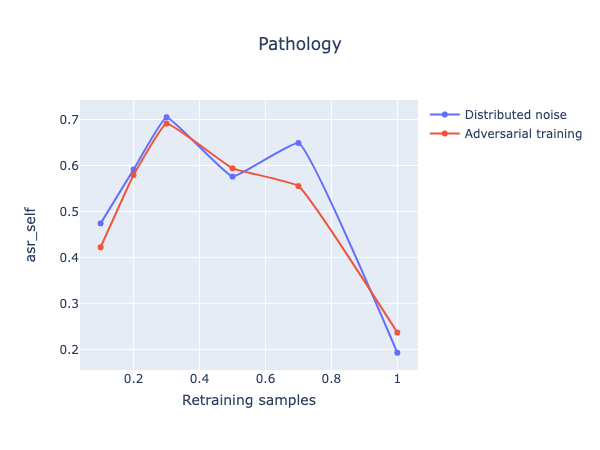
\includegraphics[width=0.6\textwidth]{newplot (15).png} 
        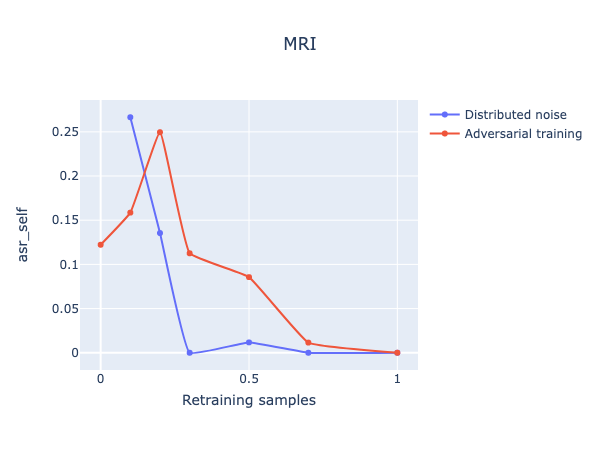
\includegraphics[width=0.6\textwidth]{newplot (13).png} \hspace{-40pt}
    \end{minipage}

    \begin{minipage}{1.21\textwidth}
        \centering
        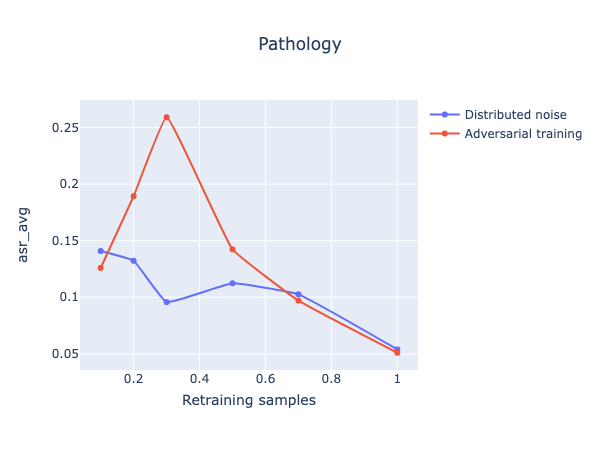
\includegraphics[width=0.6\textwidth]{newplot (16).png}
        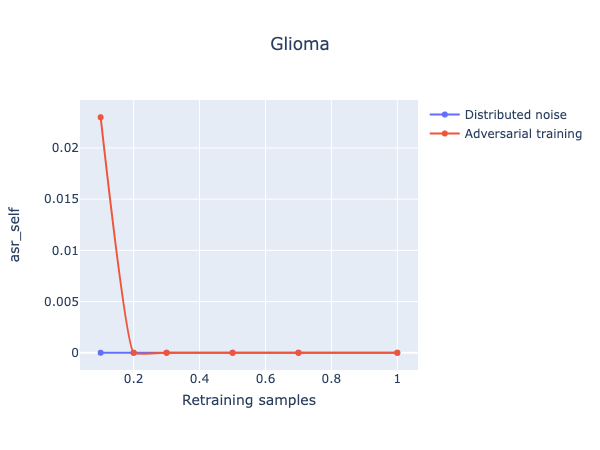
\includegraphics[width=0.6\textwidth]{newplot (11).png}\hspace{-40pt}
    \end{minipage}

    \caption{Effect of the number of adversarial samples on the average attack success rate, for benign and adversarial clients, with and without differential privacy. The results show that using more retraining samples in the global model decreased the attack success rate in all scenarios, with distributed noise outperforming adversarial training.}
    \label{fig: epsilon graphs}
\end{figure*}



\begin{figure*}[t!]
    \centering
    \begin{minipage}{1.2\textwidth} % Increase to allow more space for wider images
        \centering
        \subfloat[]{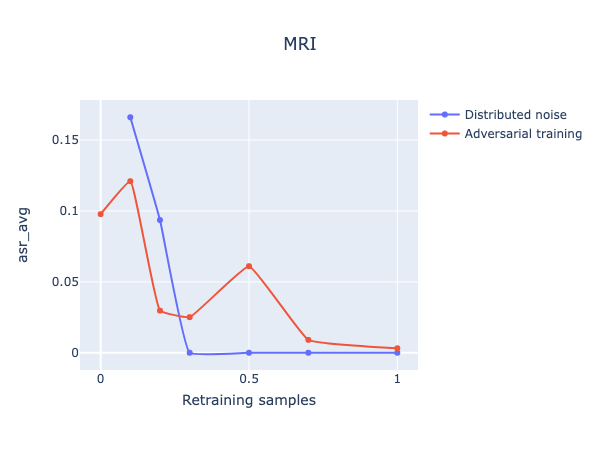
\includegraphics[width=0.38\textwidth]{newplot (14).png}}\hspace{-20pt}
        \subfloat[]{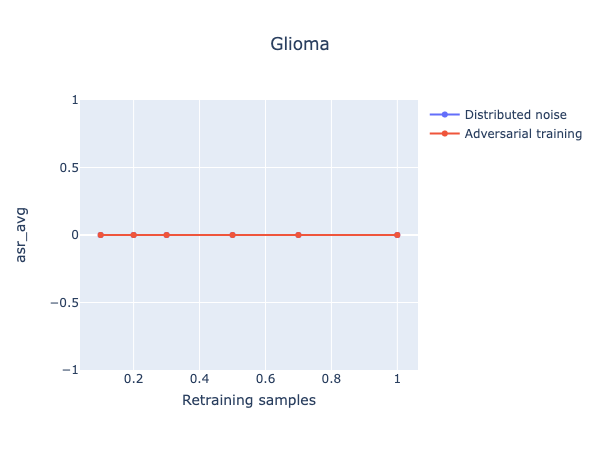
\includegraphics[width=0.38\textwidth]{newplot (12).png}}\hspace{-20pt}
        \subfloat[]{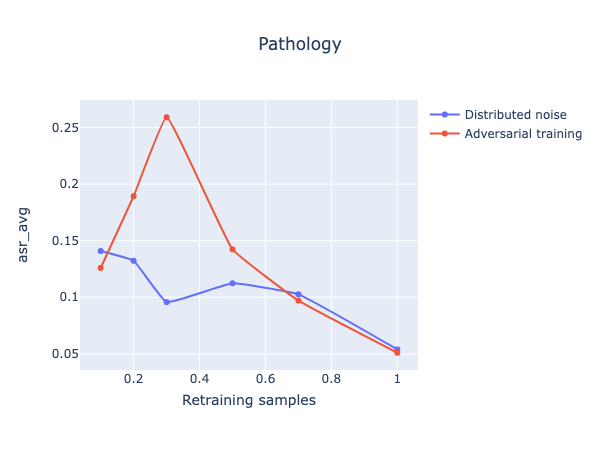
\includegraphics[width=0.38\textwidth]{newplot (16).png}}
    \end{minipage}

    \vspace{10pt} % Add some vertical space between rows

    \begin{minipage}{1.2\textwidth} % Increase to allow more space for wider images
        \centering
        \subfloat[]{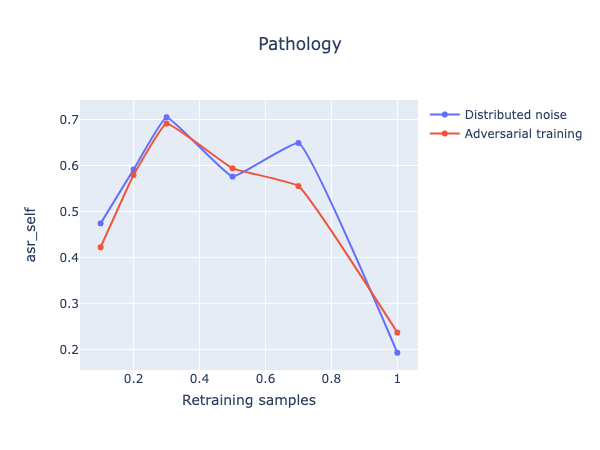
\includegraphics[width=0.38\textwidth]{newplot (15).png}}\hspace{-20pt}
        \subfloat[]{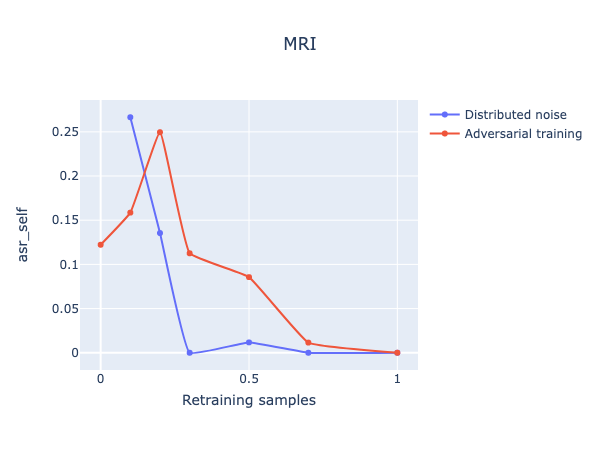
\includegraphics[width=0.38\textwidth]{newplot (13).png}}\hspace{-20pt}
        \subfloat[]{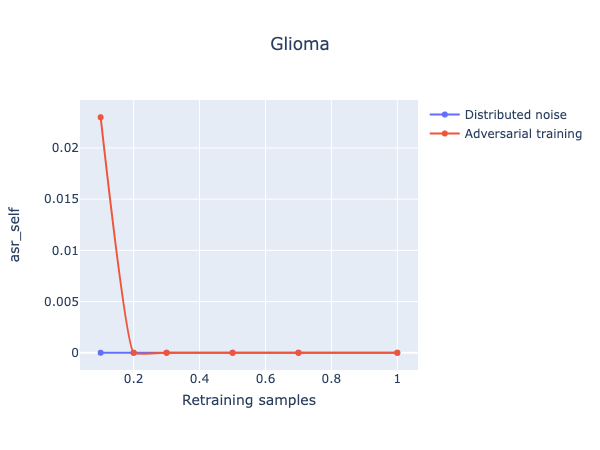
\includegraphics[width=0.38\textwidth]{newplot (11).png}}
    \end{minipage}

    \caption{Effect of the number of adversarial samples on the average attack success rate, for benign and adversarial clients, with and without differential privacy. The results show that using more retraining samples in the global model decreased the attack success rate in all scenarios, with distributed noise outperforming adversarial training.}
    \label{fig: epsilon graphs}
\end{figure*}


The results of our experiments demonstrate that distributed noise training provides a more effective defense against adversarial attacks than the adversarial training method.  Our experiments showed that using distributed noise training can reduce the attacker's self-ASR by up to 8\% and the attacker's average ASR by up to 27\%, across three different datasets. Additionally, we observed that the effectiveness of distributed noise is dependent on the step size used for the attack, with smaller steps leading to greater effectiveness. Furthermore, we found that using more retraining samples in the global model can lead to a lower attack success rate, and that the addition of differential privacy can improve defense performance. These findings are consistent with the existing literature on adversarial defenses, and concludes that  distributed noise training is a viable approach for defending against adversarial attacks.
\section{Conclusion }
\textbf{Summary }
In this paper, we present a federated learning system with robustness to adversarial attacks. To this end, we propose a distributed noise training approach, which is capable of defending against various adversarial attack scenarios. Experimental results show that our system achieves an accuracy comparable to secured baseline models, as well as better performance than both differential privacy and baseline adversarial training methods. In addition, our system provides improved security against malicious clients. Overall, our method provides a secure and effective way to defend against adversarial attacks in a federated learning setting. We believe that this work will serve as a starting point for further research on robustness in federated learning systems. We also hope that our system will be useful in real-world applications in the medical domain and beyond.
\\\textbf{Future directions}
In the future, research should focus on improving the security and privacy of federated learning through advanced defense schemes. This includes exploring methods for securely aggregating models, ensuring data privacy through differential privacy, and developing robust models by incorporating adversarial training. Additionally, more research is needed on developing strategies for defending against malicious clients, such as distributed noise training, and evaluating the transferability of attacks on different models. 
 Furthermore, methods for producing medical annotated images and larger datasets can be developed in order to provide more reliable medical learning systems. Finally, research should focus on understanding how to effectively use federated learning in medical image analysis tasks and ensure the robustness and security of the models despite the presence of adversaries.

